\documentclass[]{article}

\usepackage[nottoc,numbib]{tocbibind}

\usepackage{amssymb,amsmath}
\setcounter{tocdepth}{3}
\usepackage{graphicx}
\usepackage{algorithm, algorithmic}
\usepackage{caption}
\usepackage{complexity}
\usepackage{subcaption}
\usepackage{tabularx}
\usepackage{cite}
\usepackage{pgfgantt}
\usepackage{listings}
\usepackage{xcolor}
\definecolor{darkgreen}{rgb}{0.0, 0.6, 0.0}
\graphicspath{{images/}}
\captionsetup{compatibility=false}
\lstset{
    language=Python,
    basicstyle=\ttfamily\small,
    keywordstyle=\color{blue},
    stringstyle=\color{red},
    commentstyle=\color{darkgreen},
    showstringspaces=false,
    numbers=left,
    numberstyle=\tiny\color{gray},
    breaklines=true,
    frame=single,
    captionpos=b,
    emph={__init__}, % list function keywords or names here
    emphstyle=\color{purple} % set your preferred function name color here
}
\usepackage[colorlinks=true, linkcolor=blue, citecolor=cyan, urlcolor=cyan]{hyperref}

%\usepackage{setspace}
%%\singlespacing
%%\onehalfspacing
%\doublespacing

\DeclareMathOperator*{\argmax}{argmax}

\DeclareMathOperator*{\optimise}{optimise}
\DeclareMathOperator*{\subjectto}{subject\hspace{0.1cm}to}
%opening
\title{\textbf{AI-Driven Generative Design: Evolutionary Optimisation of Residential Floor Plans}}
\author{Zuxing Wu, a1816653\\ \\Supervisor: Adel Nikfarjam\\ \\Master of Computer Science}

\begin{document}

\maketitle\nonumber

\newpage\nonumber

\tableofcontents

\newpage

% \begin{abstract}
% Abstract
% \end{abstract}

\section{Introduction}
\subsection{Aim}
Residential floor plan design is a multifaceted and challenging task that necessitates careful consideration of factors such as room dimensions, spatial adjacency, privacy, convenience, and orientation. Conventional approaches to floor plan design are often time-consuming and labour-intensive, frequently resulting in suboptimal outcomes. Evolutionary algorithms have emerged as a promising alternative for optimising floor plans, as they are capable of efficiently exploring the design space and generating high-quality solutions. This project aims to develop an improved method for optimising residential floor plans through the application of evolutionary algorithms, addressing several limitations identified in previous research. The proposed approach utilises a novel and straightforward representation scheme, with the fitness of each floor plan evaluated according to multiple criteria, including privacy, comfort, practicality, and convenience. The findings of this research are expected to advance the field of residential floor plan design and offer valuable insights into the application of evolutionary algorithms to architectural design challenges.

\subsection{Motivation}
Residential floor plan design constitutes a fundamental component of architectural practice, encompassing the spatial arrangement of rooms, windows, doors, corridors, and ancillary spaces within a dwelling. The configuration of a floor plan profoundly influences the functionality, convenience, comfort, ventilation, and energy efficiency of a residential building. Conventional approaches to floor plan design typically rely on manual drafting or computer-aided design (CAD) tools, processes that are often both time-consuming and labour-intensive. Furthermore, such methods may yield suboptimal outcomes, as they are heavily dependent on the subjective judgment and experience of individual designers.

In contrast, evolutionary algorithms provide a systematic and effective means for optimising floor plans by thoroughly exploring the design space and generating high-quality solutions. These algorithms are inspired by the principles of natural evolution, operating on a population of candidate solutions and utilising mechanisms such as crossover and mutation to iteratively improve design quality across generations. The performance of each candidate solution is rigorously evaluated using fitness functions, which quantitatively assess the extent to which the design satisfies the specified objectives of the floor plan optimisation problem.

\section{Literature Review}
Previous research has explored the application of evolutionary algorithms to optimise residential floor plans. Brintrup et al.~\cite{10.1007/11732242_56} compared three interactive genetic algorithms (i.e., sequential IGA, multi-objective IGA, parallel IGA) on a multi-objective floor planning task, and found that the multi-objective IGA provides more diverse results and faster convergence for optimising floor plans. They developed interactive evolutionary algorithms that allow designers to incorporate their preferences and constraints into the optimisation process. This method has shown promising results in generating floor plans that meet both functional and aesthetic requirements.

It was found that proportional roulette wheel selection is the best parent selection method for the mating pool, and k-point crossover is the most effective for fitness evolutionary improvement~\cite{7844659}.
Combining evolutionary algorithms with greedy-like algorithms can help find near-optimal solutions in Automated Floor Plan Generation (AFPG), though it is a simplified model of multi-objective optimisation by linear composition of the partial evaluation functions~\cite{doi:10.1177/1478077119832982}. Subramanian et al.~\cite{9675541} used a genetic algorithm with KD tree models in a web application to generate floor plans for even non-expert users.

Wang and Duan~\cite{WANG2023100238} tried to optimise floor plan design by focusing on energy consumption and consumer satisfaction, proving that the preferences of different types of consumers differed significantly. Therefore, different evaluation criteria are needed for satisfying different family types~\cite{WANG2023100238}. The quality and efficiency of residential floor plan design can be improved by combining Monte Carlo tree search algorithm (MCTS) and particle swarm optimisation (PSO)~\cite{YAN2024110546}. The MCTS algorithm takes human experience into consideration so that it can compress the search space and improve the efficiency of the search process~\cite{YAN2024110546}. The PSO algorithm can handle continuous variables and is suitable for optimising the size of rooms due to parallel processing~\cite{YAN2024110546}.

Energy consumption, probable uniformity (PU), and spatial useful daylight illuminance (sUDI) are three objectives that are considered in Chaichi and Andaji Garmaroodi's optimisation process~\cite{CHAICHI2024108842} using NSGA-II algorithm, and the results show that the NSGA-II algorithm can provide a set of more sustainable floor plans that requires less computational power and time. Reliable metrics for evaluating the amount of light and the uniformity of light are tested in the optimisation process, and can avoid unwanted convergence because they restrict each other~\cite{CHAICHI2024108842}.

Shi et al.~\cite{10.5555/3666122.3666421} chose (1+1)-EA (Evolutionary Algorithm) to optimise macro placement by randomly selecting two macros and exchange their coordinate, which only keep one solution and iteratively improves it. Laignel et al.~\cite{LaignelGraziella2021Fpgt} proposes a novel constraint programming-genetic algorithm for automatic apartment layout generation, demonstrating its ability to produce architecturally valid floor plans within a minute by discretizing space into a grid and solving layout assignments under complex constraints.

Zou et al.~\cite{ZouDexuan2024Amsa} proposes a memory-based simulated annealing algorithm for fixed-outline floor planning with soft blocks, using a memory pool and geometric auxiliary function to escape local optima and efficiently meet design constraints, showing superior performance on benchmarks. Both Zou~\cite{ZouDexuan2024Amsa} and Singha~\cite{SinghaT.2012OoFu} used B*-tree to represent the floor plan, which is a hierarchical structure that allows for efficient storage and manipulation of the floor plan data.
Kang and Kim~\cite{KangShinjin2022Fpof} presents a novel method that analyses mobile app logs and Google server data to identify user behaviour patterns, using a genetic algorithm to generate optimal indoor floor plans that minimise living costs and enhance spatial analysis.
Zawidzki and Szklarski~\cite{ZawidzkiMachi2020Moot} developed a multi-objective optimisation framework for single-story house floor plans, balancing functionality, sunlight, view, and noise reduction through gradient-based methods and user-defined preferences, demonstrated via a case study.

Furthermore, the integration of machine learning techniques with evolutionary algorithms has gained attention in recent decades~\cite{HousseinEssamH.2021MAiP}. For example, Wang et al.~\cite{WANG20051329} proposed a hybrid approach that combines a genetic algorithm with a neural network to predict the fitness of candidate solutions. This method significantly reduces the computational cost of evaluating large populations and accelerates the optimisation process.

Overall, the literature indicates that evolutionary algorithms, particularly when combined with other optimisation techniques and machine learning methods, offer a powerful tool for optimising residential floor plans. These approaches not only improve the efficiency and quality of the designs but also provide flexibility in accommodating various design preferences and constraints.

\section{Methodology}
The methodology of this project involves the application of evolutionary algorithms to optimise residential floor plans. The process will be divided into several key stages: 1.\ Representation of the floor plan, 2.\ Solution evaluation, 3.\ Initialisation of the population, 4.\ Design of the evolutionary optimisation framework. These stages are described in detail below.

\subsection{Representation of Floor Plans}
To represent a concrete representation of the floor plan, we will use a hierarchical structure (shown in Figure~\ref{fig:representation_hierarchy}) to represent the floor plan data. The top-level structure will be a \texttt{House} class that contains a boundary and a list of rooms. Each room will be represented by a \texttt{Room} class, which includes its dimensions (width and depth), position (x, y coordinates), and lists for doors and windows. The doors and windows will be represented as tuples containing their width, the wall they are located on, and their position on that wall.
\begin{figure}[h]
    \centering
    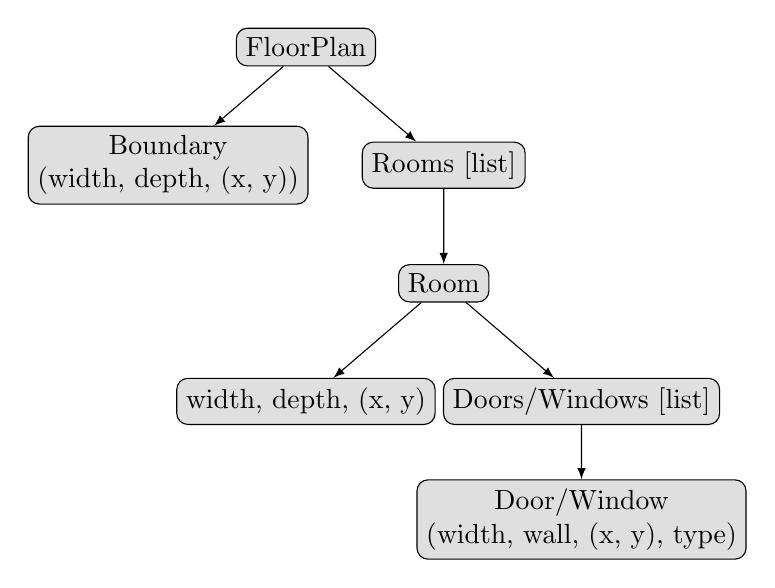
\begin{tikzpicture}[
            level distance=1.5cm,
            every node/.style={rectangle,draw,rounded corners,align=center,fill=gray!25},
            edge from parent/.style={draw,-latex},
            sibling distance=3.5cm
        ]
        \node {FloorPlan}
        child { node {Boundary\\(width, depth, (x, y))} }
        child { node {Rooms [list]}
        child { node {Room}
        child { node {width, depth, (x, y)} }
        child { node {Doors/Windows [list]}
        child { node {Door/Window\\(width, wall, (x, y), type)} }
        }
        }
        };
    \end{tikzpicture}
    \caption{Hierarchical representation of the floor plan data structure.}
    \label{fig:representation_hierarchy}
\end{figure}

To display the floor plan, we used Python's \texttt{matplotlib} library to create and save a visual representation of the floor plan. We defined a \texttt{save\_snapshots} function that takes a layout as one of the parameters, and generates a visual representation of the floor plan. The function iterates through each room in the layout, draws rectangles for the rooms, and adds doors and windows as lines on the walls. The boundary is drawn in black. The resulting image is saved as a PNG file.

\subsection{Solution Evaluation}
Fitness functions will evaluate each floor plan mainly based on these 4 criteria:
privacy, comfort, practicality, convenience. We created 24 fitness functions based on Wang and Duan's evaluation indicators~\cite{WANG2023100238} along with professional's advice. Our fitness functions are shown in Table~\ref{tab:fitness_functions}.
\begin{table}[h]
    \centering
    \caption{List of 24 Fitness Functions (Dark green means eventually being used)}
    \label{tab:fitness_functions}
    \begin{tabularx}{\textwidth}{l l}
        \hline
        \textbf{Function Name}                         & \textbf{Description}                           \\
        \hline
        dis\_MBR\_BR                                   & Distance between Main Bedroom and Bedroom      \\
        dis\_MBR\_BA                                   & Distance between Main Bedroom and Bathroom     \\
        \textcolor{darkgreen}{check\_LR\_orientation}  & Living Room orientation check                  \\
        check\_DR\_natural\_light                      & Dining Room natural light check                \\
        ventilation                                    & Ventilation evaluation                         \\
        north\_facing\_area                            & North-facing area calculation                  \\
        percentage\_hall                               & Percentage of hall area                        \\
        percentage\_balcony                            & Percentage of balcony area                     \\
        \textcolor{darkgreen}{utilization\_rate }      & Utilization rate of the floor plan             \\
        dis\_BR\_BA                                    & Distance between Bedroom and Bathroom          \\
        dis\_BA\_LR\_door                              & Distance between Bathroom and Living Room door \\
        \textcolor{darkgreen}{check\_GAR\_side}        & Garage should be on the same side as the entry \\
        \textcolor{darkgreen}{dis\_KIC\_LR}            & Distance between Kitchen and Living Room       \\
        \textcolor{darkgreen}{dis\_KIC\_DR}            & Distance between Kitchen and Dining Room       \\
        \textcolor{darkgreen}{dis\_LR\_DR}             & Distance between Living Room and Dining Room   \\
        \textcolor{darkgreen}{check\_no\_entry\_touch} & Entry not touching other closed rooms check    \\
        \textcolor{darkgreen}{cal\_overlap\_rate}      & Overlap rate calculation                       \\
        \textcolor{darkgreen}{diff\_public\_private}   & Differentiate private rooms from public rooms  \\
        \textcolor{darkgreen}{check\_KIC\_orientation} & Kitchen orientation check                      \\
        \textcolor{darkgreen}{dis\_LDR\_KIC}           & Distance between Laundry and Kitchen           \\
        \textcolor{darkgreen}{dis\_GAR\_KIC}           & Distance between Garage and Kitchen            \\
        \textcolor{darkgreen}{dis\_MBR\_LR}            & Distance between Main Bedroom and Living Room  \\
        \textcolor{darkgreen}{dis\_MBR\_KIC}           & Distance between Main Bedroom and Kitchen      \\
        \textcolor{darkgreen}{bigger\_MBR}             & Main Bedroom area $>$ other bedroom area       \\
        \hline
    \end{tabularx}
\end{table}

The straight distance between the geometric centres of room $m$ and $n$ is defined as:
\begin{equation*}
    \text{dis}(m, n) = \sqrt{(x_m - x_n)^2 + (y_m - y_n)^2}
\end{equation*}
but at the late stage of the optimisation process, this distance is calculated through \texttt{polygon.distance()} function from the \texttt{shapely} library, which is more accurate and convenient than the above formula.

The percentage of area of $R$ to the interior area of the floor plan is defined as:
\begin{equation*}
    \% \text{ of } R = \left( \frac{\text{Area of } R}{\text{Interior Area of Floor Plan}} \right) \times 100\%
\end{equation*}

The utilisation rate of a house is defined as the percentage of occupied area to the total area of the floor plan:
\begin{equation*}
    \text{utilisation Rate} = \left( \frac{\text{Occupied Area}}{\text{Total Area}} \right) \times 100\%
\end{equation*}
The overlap rate is defined as the percentage of overlapping area to the total area of the floor plan:
\begin{equation*}
    \text{overlap Rate} = \left( \frac{\text{Overlapping Area}}{\text{Sum All Rooms Area}} \right) \times 100\%
\end{equation*}
The differentiation between public and private rooms is based on the classification of rooms into public (e.g., living room, dining room, kitchen, garage and laundry) and private (e.g., bedrooms, bathrooms). The differentiation is evaluated based on the comparison of distance between these rooms and the entry. All public rooms should be close to the entry, while private rooms should be further away. The differentiation is calculated as:
\begin{equation*}
    \text{diff\_public\_private} = \frac{1}{|P| \cdot |Q|} \sum_{p \in P} \sum_{q \in Q} \mathbb{I}\left( d(\text{entry}, p) < d(\text{entry}, q) \right)
\end{equation*}
where $P$ is the set of public rooms, $Q$ is the set of private rooms, $d(\text{entry}, r)$ denotes the distance from the entry to the centre of room $r$, and $\mathbb{I}(\cdot)$ is the indicator function that returns 1 if the condition is true and 0 otherwise. This metric measures the proportion of public-private room pairs where the public room is closer to the entry than the private room, thus quantifying the spatial differentiation between public and private spaces.

These proposed methods are implemented in Python. All fitness values are calculated and normalised to a range of 0 to 1, where higher values indicate better performance. The evaluation process involves calculating the fitness values for each floor plan in the population and selecting the best individuals for particles updating their velocity and position in PSO.

\subsection{Population Initialisation}
The first step in the evolutionary process is to generate an initial population of residential floor plans. The initialisation process involves generating a set of random rooms and arranging them into a floor plan layout, subject to the following constraints and parameter ranges:

\begin{itemize}
    \item \textbf{House boundary:} width = 15\,m, depth = 8\,m.
    \item \textbf{Entry:} a line segment at the boundary, $\texttt{LineString([(0, 4), (0, 5)])}$.
    \item \textbf{8 Room types and size ranges:}
          \begin{itemize}
              \item Garage (\texttt{GAR}): width 5--6\,m, depth 3--6\,m
              \item Laundry Room (\texttt{LDR}): width 3\,m, depth 3\,m
              \item Dining Room (\texttt{DR}): width 3--5\,m, depth 3--5\,m
              \item Living Room (\texttt{LR}): width 3--6\,m, depth 3--6\,m
              \item Kitchen (\texttt{KIC}): width 3--4\,m, depth 3--4\,m
              \item Main Bedroom (\texttt{MBR}): width 3--6\,m, depth 3--6\,m
              \item Bedroom1 (\texttt{BR1}): width 3--5\,m, depth 3--5\,m
              \item Bathroom (\texttt{BA}): width 2--4\,m, depth 2--4\,m
          \end{itemize}
    \item \textbf{Window width:} 0.5--1.5\,m
    \item \textbf{Door width:} 0.8--1.5\,m
\end{itemize}

The rooms are assigned random sizes within the specified ranges and placed within the house boundary. The initialisation strategy is designed to produce a diverse set of floor plans that serve as a starting point for the evolutionary optimisation process. At the late stage of our research, we only need to randomly generate a single floor plan, which will be mutated and evaluated continuously so as to evolve the floor plan towards an optimal solution.

\subsection{Evolutionary Optimisation Framework}
The evolutionary optimisation framework initially was based on particle swarm optimisation (PSO) algorithm, which is suitable for optimising the size of rooms due to parallel processing, and Monte Carlo Tree Search (MCTS) algorithm which can handle discrete variables (i.e., room position)~\cite{YAN2024110546}. In our implementation, the width and depth are integer values, which means we are using discrete binary particle swarm optimisation (BPSO) algorithm~\cite{YAN2024110546, KennedyJ.1997Adbv}. The topology of this type PSO algorithm is a von Neumann topology~\cite{HousseinEssamH.2021MAiP}, where each particle is connected to its neighbours in a grid-like structure. The PSO algorithm updates the velocity and position of each particle based on its own best position and the best position of its neighbours. The velocity update equation is given by:
\begin{equation*}
    v_i(t+1) = w(t) \cdot v_i(t) + c_1 \cdot r_1 \cdot (p_i - x_i(t)) + c_2 \cdot r_2 \cdot (g - x_i(t))
\end{equation*}
where $v_i(t)$ is the velocity of particle $i$ at time $t$, $w(t)$ is the inertia weight, $c_1$ and $c_2$ are the cognitive and social coefficients, respectively, $r_1$ and $r_2$ are random numbers uniformly distributed in [0, 1], $p_i$ is the best position of particle $i$, and $g$ is the global best position among all particles.

However, the MCTS algorithm did not optimise the room position very well, so it was replaced by a simple greedy algorithm called (1+1) Evolutionary Algorithm (EA). The (1+1) EA algorithm (see Algorithm~\ref{alg:1+1-ea-position}) is a simple evolutionary algorithm that maintains a single individual and applies mutation to generate new individuals. The PSO algorithm will be used to optimise the size of rooms, while the (1+1) EA will be used to optimise the room position. The framework will involve the application of genetic operators, such as randomly add or minus a small perturbation to the current room size, swap two random rooms, and so on, to generate new floor plans from the existing population. The optimisation process will be repeated for a specified number of generations or until a termination criterion is met.

\begin{algorithm}[H]
    \caption{: (1+1) EA for Mutating Room Positions}
    \label{alg:1+1-ea-position}
    \begin{algorithmic}[1]
        \REQUIRE Boundary, List of Rooms, Maximum Iterations $max\_iter$
        \STATE Initialise \texttt{placed\_rooms} by randomly placing each room at a legal position within the boundary
        \STATE Set \texttt{best\_layout} $\gets$ layout with \texttt{placed\_rooms}
        \STATE Set \texttt{best\_fitness} $\gets$ fitness of \texttt{best\_layout}
        \FOR{$j = 1$ to $max\_iter$}
        \FOR{each room $i$ in \texttt{placed\_rooms}}
        \STATE Generate a random number $r \in [0,1]$
        \IF{$r < 0.05$}
        \STATE Randomly select a new legal position for room $i$
        \STATE Create a new layout by moving room $i$ to the new position
        \STATE Compute fitness of the new layout
        \IF{new fitness $>$ \texttt{best\_fitness}}
        \STATE Update \texttt{best\_layout} and \texttt{best\_fitness}
        \STATE Update \texttt{placed\_rooms} with the new position for room $i$
        \ENDIF
        \ENDIF
        \ENDFOR
        \ENDFOR
        \RETURN \texttt{best\_layout}, \texttt{best\_fitness}
    \end{algorithmic}
\end{algorithm}

Later, the PSO algorithm was replaced by the (1+1) EA as well, so that the room sizes (i.e., width and depth) could be optimised in a similar way to the room position (see Algorithm~\ref{alg:1+1-ea-size}). The (1+1) EA algorithm randomly selects a room in the floor plan and generates a new room size by adding or subtracting a small random perturbation to the current size. The new room size is evaluated using the same fitness functions, and if it results in a better fitness value, it replaces the current best room size. This process continues until all rooms have been assigned their optimal sizes.
\begin{algorithm}[H]
    \caption{: (1+1) EA for Mutating Room Sizes}
    \label{alg:1+1-ea-size}
    \begin{algorithmic}[1]
        \REQUIRE Boundary, Room Size Ranges, Maximum Iterations $max\_iter$
        \STATE Randomly generate initial room sizes within the specified ranges
        \STATE Set \texttt{best\_layout\_rooms} $\gets$ initial room sizes
        \STATE Set \texttt{best\_fitness} $\gets -\infty$
        \FOR{$i = 1$ to $max\_iter$}
        \STATE Copy \texttt{best\_layout\_rooms} to \texttt{rooms}
        \FOR{each room $j$ in \texttt{rooms}}
        \STATE Generate a random number $r \in [0,1]$
        \IF{$r < 0.125$}
        \STATE Mutate width and depth of room $j$ by adding random integers in $[-3, 3]$, keeping within allowed range
        \ENDIF
        \ENDFOR
        \STATE Use \texttt{Position\_OnePlusOneEA} to optimise positions for current sizes, get \texttt{best\_layout}, \texttt{fitness}
        \IF{\texttt{fitness} $>$ \texttt{best\_fitness}}
        \STATE Update \texttt{best\_layout}, \texttt{best\_fitness}, \texttt{best\_layout\_rooms}
        \ENDIF
        \STATE Record \texttt{best\_fitness} in history
        \ENDFOR
        \RETURN \texttt{best\_layout}, \texttt{best\_fitness}
    \end{algorithmic}
\end{algorithm}

If possible, other optimisation algorithms, such as simulated annealing algorithm or differential evolution, will be explored to further enhance the optimisation process. The final output of the evolutionary optimisation framework will be an optimised residential floor plan with high fitness value that meets the specified design criteria and constraints.


\section{Plan vs Progress}
\subsection{Research Plan}
My research plan consists of four main phases through the whole research.
\begin{itemize}
    \item Phase 1
          \begin{enumerate}
              \item Solution representation
              \item Solution evaluation
          \end{enumerate}
    \item Phase 2
          \begin{enumerate}
              \item Population initialisation
              \item Evolutionary optimisation
          \end{enumerate}
\end{itemize}
Each phase involves specific tasks and activities that will be carried out over a period of 6 months (since I did not make a plan for semester 1 of this year). The timeline for the research plan, at that time, is shown in the Gantt chart below. \\
\begin{ganttchart}[
        hgrid,
        vgrid,
        x unit = 1.4cm,
        y unit chart=0.7cm,
        title/.append style={fill=none},
        title label font=\bfseries\footnotesize,
        title label anchor/.append style={below=-1.6ex},
        include title in canvas=false,
        bar label font=\normalsize\scshape,
        bar label node/.append style={left=2ex},
        bar/.append style={fill=yellow!60},
        group/.append style={fill=cyan!80},
        bar incomplete/.append style={fill=red!30},
        progress label text={},
        group right shift=0,
        group top shift=0.7,
        group height=.3
    ]{1}{6}
    \gantttitle{2024.09--2025.02}{6} \\
    \gantttitlelist{9,10,11,12,1,2}{1} \\
    \ganttgroup{Phase 1}{1}{3} \\
    \ganttbar{Representation}{1}{2} \\
    \ganttbar{Evaluation}{2}{3} \\
    \ganttgroup{Phase 2}{4}{6} \\
    \ganttbar{Optimization}{4}{5} \\
    \ganttbar{Initialization}{5}{6}
    \gantttitle{Last Semester Research Plan Timeline}{6} \\
\end{ganttchart}

However, the real research progress did not go as planned. The research plan was adjusted to focus on the solution evaluation and evolutionary optimisation. The solution evaluation is the key to the quality of the generated floor plans, and the evolutionary optimisation is the core of this research. The solution representation is the prerequisite of solution evaluation. The population initialisation can be adjusted according to the progress of the research. The true timeline for the research progress is shown in the Gantt chart below. (Orange means current semester.)\\
\begin{ganttchart}[
        hgrid,
        vgrid,
        x unit = 1.0cm,
        y unit chart=0.7cm,
        title/.append style={fill=none},
        title label font=\bfseries\footnotesize,
        title label anchor/.append style={below=-1.6ex},
        include title in canvas=false,
        bar label font=\normalsize\scshape,
        bar label node/.append style={left=0.1ex},
        bar/.append style={fill=yellow!60},
        group/.append style={fill=cyan!80},
        bar incomplete/.append style={fill=red!30},
        progress label text={},
        group right shift=0,
        group top shift=0.7,
        group height=.3
    ]{1}{9}
    \gantttitle{2024.09--2025.05}{9} \\
    \gantttitlelist{9,10,11,12,1,2}{1}
    \gantttitlelist[title/.append style={fill=orange}]{3,4,5}{1} \\
    \ganttgroup{Phase 1}{1}{3} \\
    \ganttbar{Representation}{1}{2} \\
    \ganttbar[bar/.append style={fill=brown!60}]{Evaluation}{2}{9} \\
    \ganttgroup{Phase 2}{4}{9} \\
    \ganttbar[bar/.append style={fill=brown!60}]{Optimization}{4}{9} \\
    \ganttbar{Initialization}{4}{7}
    \gantttitle{Real Research Progress}{9} \\
\end{ganttchart}


\subsection{Progress}
It can be seen from the Gantt chart above that the research process has been adjusted to mainly focus on the solution evaluation and evolutionary optimisation.

Last summer holiday, I have completed the solution representation and solution evaluation, respectively using self-defined classes to represent the floor plan and using a set of fitness functions to evaluate each floor plan. All the fitness values are calculated and normalised to a range of 0 to 1.

Fitness functions are designed to evaluate the quality of the generated floor plans based on various criteria, such as privacy, comfort, practicality, and convenience. The evaluation process involves calculating the fitness values for each floor plan in the population and selecting the best individuals for particles updating their velocity and position in PSO.

\subsubsection{PSO algorithm + MCTS algorithm}
From the start of semester 1 of 2025, I have been working on the evolutionary optimisation process. Initially, I focused on the PSO algorithm, which is suitable for optimising the size of rooms due to parallel processing, and MCTS algorithm, which handles discrete variables (i.e., room position). I had implemented the PSO algorithm and MCTS algorithm in Python, and I tried integrating them into a single framework. The integration process involves combining the two algorithms to create a hybrid optimisation approach that can effectively handle both continuous and discrete variables in the floor plan design process.

\subsubsection{MCTS algorithm replaced by (1+1) EA}
However, the integration process has proven to be more complex than anticipated, and the MCTS algorithm did not optimise the room position very well. It cannot eliminate overlap even after 2000 iterations (see Figure~\ref{fig:mcts_overlap}) (bold black line means entry).

\begin{figure}[h]
    \centering
    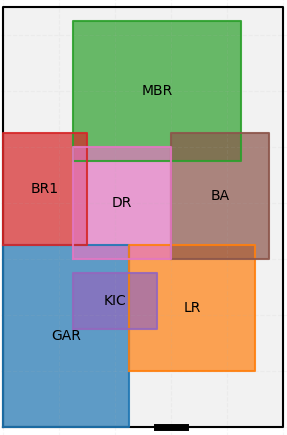
\includegraphics[width=0.4\textwidth]{images/pso-mcts-1.png}
    \caption{Example of room overlap after 2000 PSO-MCTS iterations. (Bold black line is the entry.)}
    \label{fig:mcts_overlap}
\end{figure}

Therefore, I changed it to a simple greedy algorithm called (1+1) Evolutionary Algorithm, which is a simple evolutionary algorithm that maintains a single individual and applies mutation to generate new individuals. The (1+1) EA algorithm is easier to implement and can be used to optimise the room position (i.e., the (x, y) coordinates) in the floor plan design process. If the new solution has a better fitness value, it replaces the current solution. This process continues until a termination criterion, such as a maximum number of iterations or a satisfactory fitness value, is met. It is a simple yet effective optimisation algorithm that can be used to improve the quality of the generated floor plans, especially in terms of room position.

\subsubsection{Swap two random rooms}
From this point onwards, swap mutation was adopted to optimise room positions. Swap mutation involves randomly selecting two rooms and exchanging their positions. This operation is simple yet effective, allowing the exploration of a larger design space and the generation of new floor plan solutions. The newly generated floor plan is evaluated using the same fitness functions, and if it achieves a higher fitness value, it replaces the current best solution. The results (see Figure~\ref{fig:swap-rooms}) show this can help reduce the overlap rate and improve the overall quality of the floor plans.

\begin{figure}[h]
    \centering
    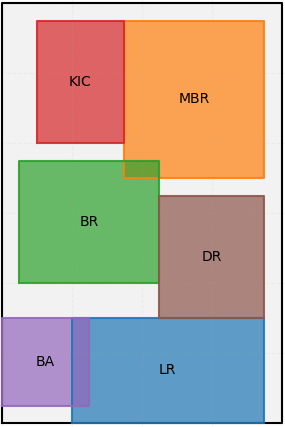
\includegraphics[width=0.4\textwidth]{images/swap-rooms.png}
    \caption{Less room overlap after using swap mutation.}
    \label{fig:swap-rooms}
\end{figure}

\subsubsection{Tune inertia weight}
In the PSO algorithm, the inertia weight plays a crucial role in balancing exploration and exploitation. Initially, I implemented a linearly decreasing inertia weight, which reduces the inertia weight from a maximum value to a minimum value over the course of iterations. However, after conducting experiments, I found that a non-linearly decreasing inertia weight performs better in terms of convergence speed and solution quality.

The non-linearly decreasing inertia weight~\cite{HousseinEssamH.2021MAiP} is defined as:
\begin{equation*}
    w(t) = w_{\text{max}} + (w_{\text{min}} - w_{\text{max}}) \cdot \left(1 - \frac{t}{T}\right)^n
\end{equation*}
where $w(t)$ is the inertia weight at iteration $t$, $w_{\text{max}}$ and $w_{\text{min}}$ are the maximum and minimum inertia weights, $T$ is the total number of iterations, and $t$ is the current iteration. $t$ is the nonlinear modulation index in the range of [0.9, 1.3].

This non-linear decrease allows the algorithm to explore the search space more effectively in the early stages and focus on exploitation in the later stages. The quadratic term ensures a smoother transition, which helps in avoiding premature convergence and improves the overall performance of the optimisation process.

\subsubsection{Prioritized fitness calculation}
To improve the performance of the optimisation process, a prioritised fitness calculation strategy has been adopted. This strategy evaluates the fitness of floor plans based on the priority of the criteria, starting with the most important and moving to the less important ones. The prioritised fitness calculation process is outlined as follows:

\begin{enumerate}
    \item \textbf{Define Priorities:} Assign a priority level to each criterion (e.g., privacy, practicality, comfort, convenience). Higher priority criteria are evaluated first. For example, the garage should be on the same side as the entry, and the main bedroom should be larger than other bedrooms. If these criteria are not met, a penalty will be deducted from the final fitness value.
    \item \textbf{Sequential Evaluation:} Calculate the fitness values for each criterion in the order of their priority. For example, overlap rate is evaluated before utilization rate. This means that if a floor plan fails to meet the zero overlap rate, it will not be evaluated for utilization rate. As can be seen in Figure~\ref{fig:prioritized-fitness}, the floor plan with zero overlap rate is evaluated for utilization rate, while the floor plan with non-zero overlap rate is not evaluated for utilization rate. Later, the privacy criterion is evaluated before the overlap rate optimisation.
          \begin{figure}[h]
              \centering
              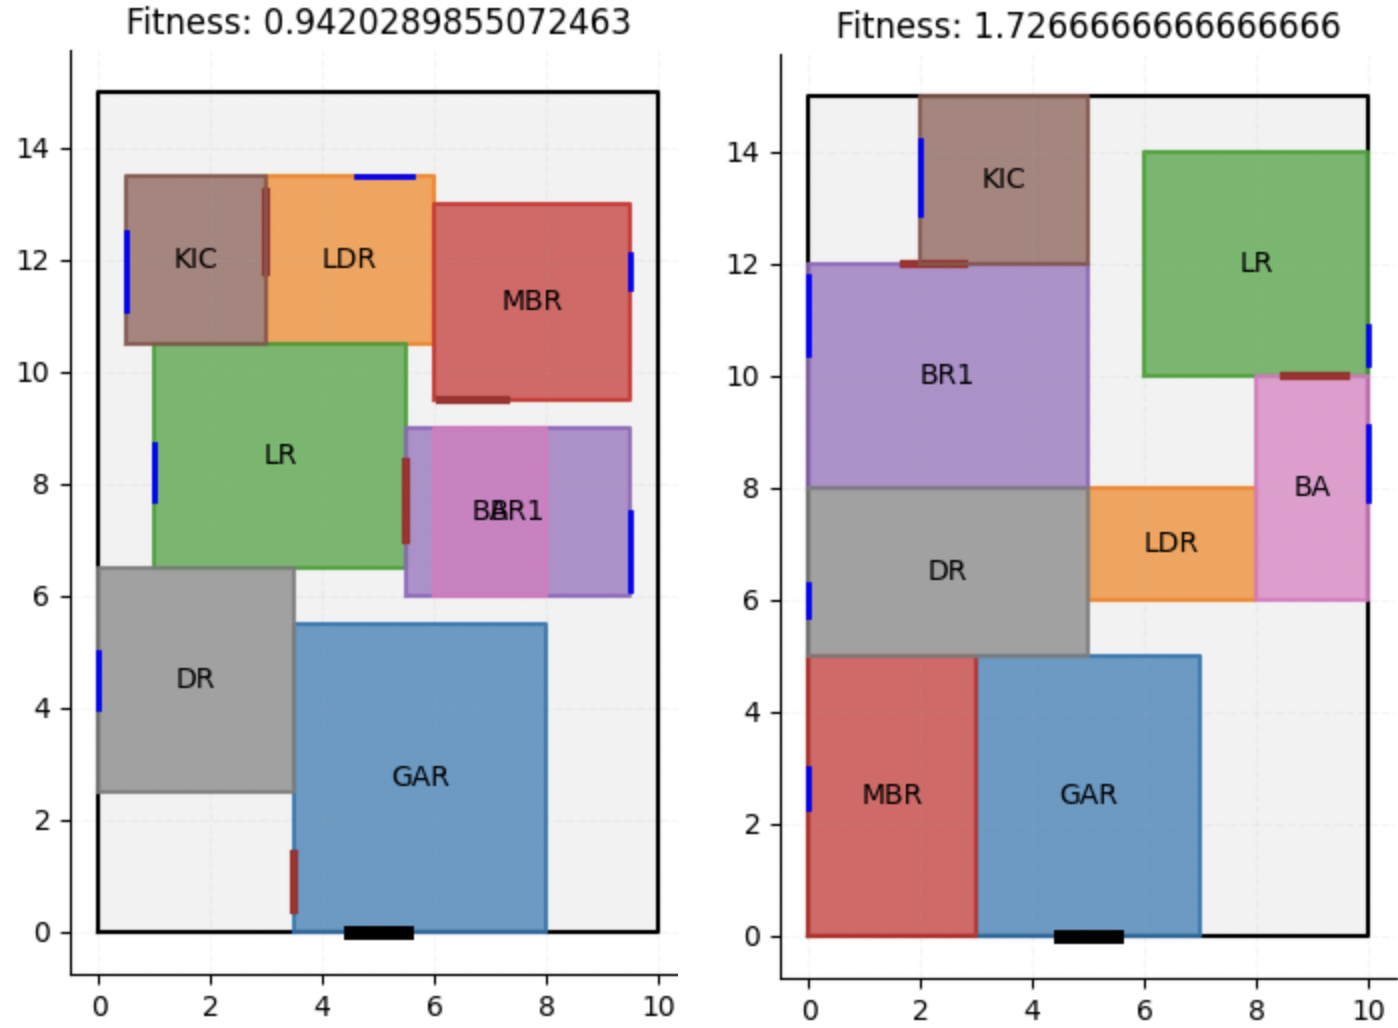
\includegraphics[width=0.9\textwidth]{images/prioritized-fitness.png}
              \caption{Example of prioritised fitness calculation. The left one is still working on reducing overlap rate. Utilization rate is only calculated for floor plans with zero overlap rate (the right one). (Bold blue lines are windows; bold brown lines are doors)}
              \label{fig:prioritized-fitness}
          \end{figure}

    \item \textbf{Weighted Aggregation:} Combine the rest of fitness values using a weighted sum, where the weights correspond to the significance levels. The overall fitness value is given by:
          \begin{equation*}
              \text{Fitness}_{\text{total}} = \sum_{i=1}^{n} w_i \cdot \text{Fitness}_i
          \end{equation*}
          where $w_i$ is the weight for criterion $i$, and $\text{Fitness}_i$ is the fitness value for criterion $i$.
    \item \textbf{Early Termination:} If a floor plan fails to meet the minimum threshold for a high-priority criterion, it is discarded without evaluating the lower-priority criteria. This reduces unnecessary computations and speeds up the optimisation process.
\end{enumerate}

This strategy ensures that the optimisation process focuses on the most critical aspects of the floor plan design, improving both efficiency and the quality of the solution generation.
It allows for a more efficient evaluation process, since it avoids unnecessary calculations in the early stages.

\subsubsection{Change land size and orientation}
In the initial version of the code, the land size and orientation were fixed, which limited the flexibility of the design process. To enhance the adaptability of the floor plan generation, I have modified the code to allow for variable land sizes and orientations. This change enables the optimisation process to spot potential problems and explore a wider range of design possibilities, accommodating different land configurations and orientations. The new approach allows for more diverse and flexible floor plan designs, making it easier to meet the needs and preferences of specific users.

\subsubsection{Remove windows and doors}
In the previous version of the code, the windows and doors were added to each room immediately after the floor plan was generated no matter whether overlap exists or not. However, this approach led to a significant increase in the complexity of the optimisation process, as the presence of windows and doors added additional constraints to the evaluation. As a result, the optimisation process became slower and less efficient, and the overall quality of the generated floor plans was not satisfactory even after 2000 iterations.
To address this issue, I have removed the windows and doors from the early generation process. Instead, the optimisation process will focus on generating the basic layout of the floor plan, including room sizes, positions, and an entry, without any additional features. Once the optimisation process is completed and a satisfactory floor plan has been generated, windows and doors can be added to the floor plan. This approach simplifies the optimisation process and allows for more efficient exploration of the design space at the early stages.

\subsubsection{PSO algorithm replaced by (1+1) EA}
After that, we found that the PSO algorithm is not suitable for optimising the size of rooms, because it always gets trapped at a local optimum and can hardly break through it. It also takes a huge amount of time to complete one iteration through all particles. Therefore, I changed it to (1+1) EA too, so that the room size (i.e., width and depth) can be optimised in a similar way to the room position optimisation. The (1+1) EA algorithm will randomly select a room in the floor plan and generate a new room size by adding or deducting a small random perturbation to the current size. The new room size will be evaluated using the fitness functions, and if it results in a better fitness value, it will replace the current best room size. This process continues until all rooms have been assigned their optimal sizes.

\subsubsection{Dotted line for open space}
In the earlier design phase, the open space in the floor plan was represented by a solid line, which made it difficult to distinguish between open space and closed rooms (e.g., dining room, living room, and kitchen. See Figure~\ref{fig:open-space-dotted-line}). To improve the clarity of the design, I have changed the representation of open space to dotted lines. This change allows for a clearer visualisation of the floor plan, making it easier to identify open spaces from other rooms in the house.
\begin{figure}[h]
    \centering
    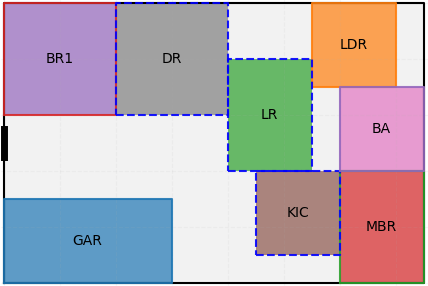
\includegraphics[width=0.6\textwidth]{images/dotted-line.png}
    \caption{Example of open space surrounded by dotted line.}
    \label{fig:open-space-dotted-line}
\end{figure}

\subsubsection{Tune weights for fitness functions}
In the final stages of the optimisation process, I have been tuning the weights of the fitness functions to achieve better results. The weights are used to balance the importance of different criteria in the evaluation process. By adjusting the weights, I can prioritise certain aspects of the design, such as low overlap or high utilization rate, to achieve better overall results. This tuning process is iterative and may require multiple rounds of testing and evaluation to find the optimal balance for the specific design goals.

\section{Experimental Results}
From the line chart in Figure~\ref{fig:compare-3algorithm}, it can be seen that the fitness value of the floor plan has been improved significantly after about 2000 iterations using PSO-(1+1) EA and dual (1+1) EA, except PSO-MCTS.\@ When running the PSO-MCTS algorithm, the fitness value gets stuck at 2.7, which means it is struggling on reaching an utilisation rate of 0.8. It cannot break through the local optimum even after 30000 iterations.
\begin{figure}[h]
    \centering
    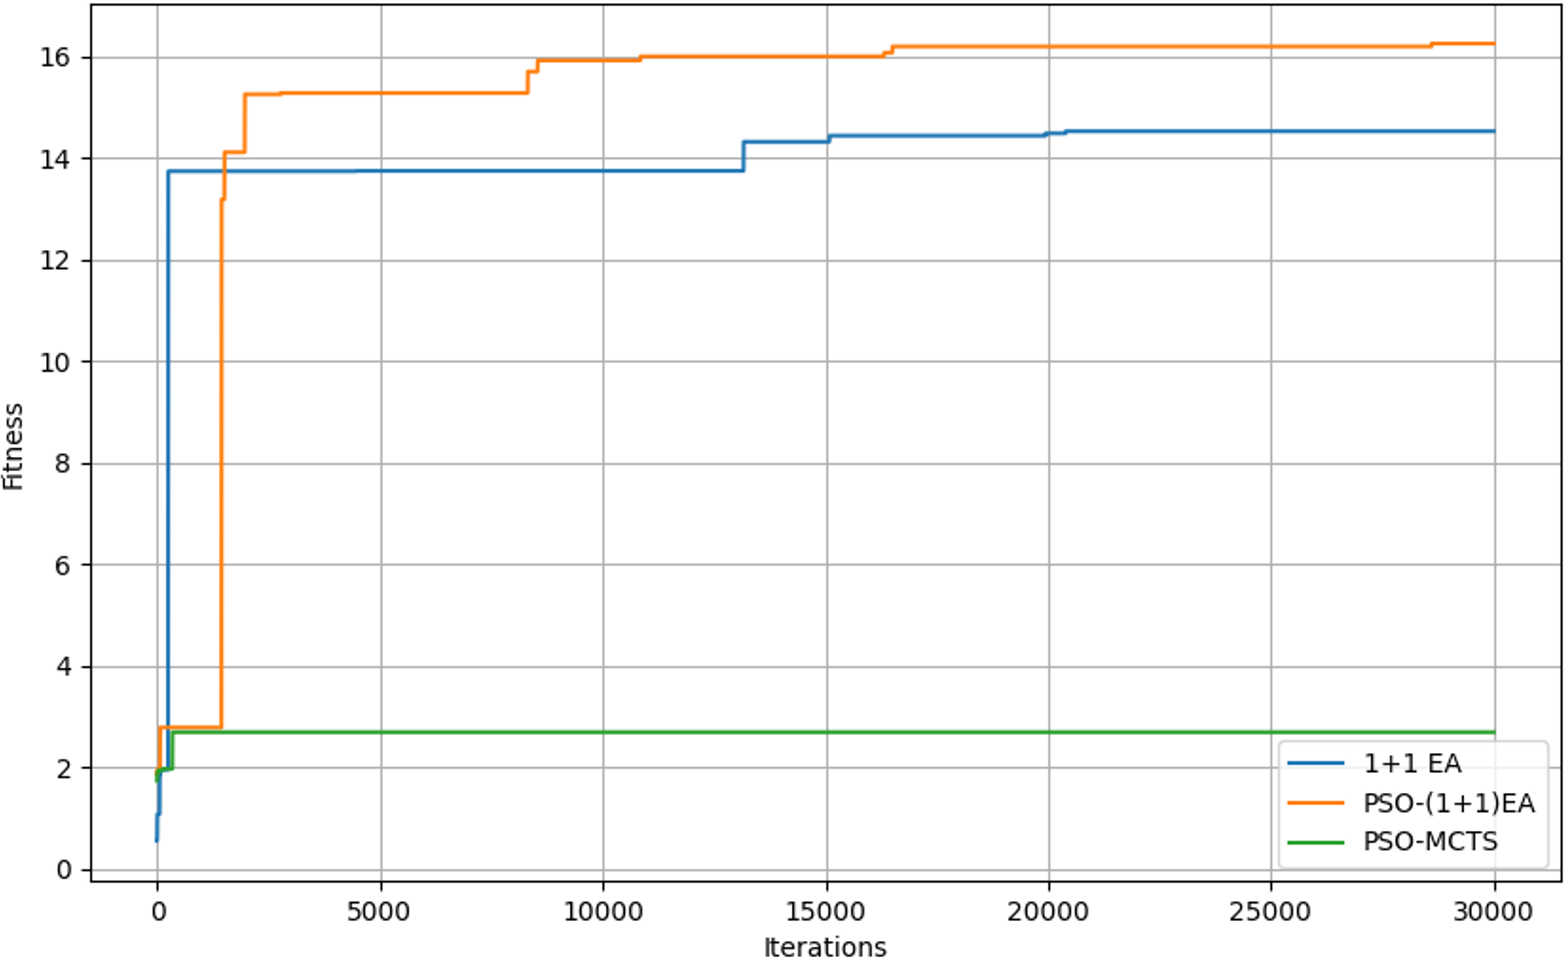
\includegraphics[width=0.8\textwidth]{images/compare-3algorithm.png}
    \caption{Fitness comparison between 3 Algorithm Combinations.}
    \label{fig:compare-3algorithm}
\end{figure}

The PSO-(1+1) EA algorithm attains a fitness value of 16.26 after 30,000 iterations, whereas the dual (1+1) EA approach surpasses a fitness value of 2.8 in a shorter duration compared to the PSO-based method, and can generate a good-enough floor plan in less than 2000 iterations (Table~\ref{tab:algorithm_comparison}). Consequently, the dual (1+1) EA algorithm is identified as the most effective strategy for floor plan optimisation in this study.
\begin{table}[h]
    \centering
    \caption{Comparison of Execution Time and Best Fitness}
    \label{tab:algorithm_comparison}
    \begin{tabularx}{\textwidth}{l | l | l}
        \hline
        \textbf{Method}      & \textbf{Execution Time} & \textbf{Best Fitness} \\
        \hline
        (1+1) EA -- (1+1) EA & 22 min 31 sec           & 14.53                 \\
        PSO--(1+1) EA        & 42 hr 19 min 30 sec     & 16.26                 \\
        PSO--MCTS            & 133 hr 33 min 30 sec    & 2.7                   \\
        \hline
    \end{tabularx}
\end{table}

\section{Conclusion}
In this thesis, I have presented the progress of my research on optimising residential floor plans using evolutionary algorithms. The research focuses on the representation of floor plans, evaluation of solutions, and the application of evolutionary optimisation techniques. The initial plan was to use a combination of PSO and MCTS algorithms, but due to the limitations of the MCTS algorithm in optimising room positions, I switched to a (1+1) EA approach. The optimisation process has shown promising results, with significant improvements in fitness values after 2000 iterations.
The final results indicate that the dual (1+1) EA algorithm is the most effective strategy for floor plan optimisation, achieving a fitness value of 14.53 in 23 minutes. The research has demonstrated the potential of evolutionary algorithms in generating high-quality residential floor plans that meet various design criteria and constraints.

\section{Future Work}
Future work will focus on further enhancing the optimisation process by exploring additional evolutionary algorithms to improve the quality of the generated floor plans and develop a robust framework for real-world applications.

Planned improvements include:
\begin{itemize}
    \item Filling blank areas or moving rooms to one side to improve space utilization and layout efficiency.
    \item Explicitly representing corridors in the floor plan to ensure better connectivity and circulation.
    \item Incorporating corridors, doors, and windows into the evaluation process, so their placement and properties are considered in the fitness calculation.
    \item Applying other algorithms, such as simulated annealing and differential evolution, to further explore the solution space and escape local optima.
\end{itemize}


\section{Plagiarism Declaration}
I hereby declare that this submission is my own work and to the best of my knowledge, it contains no material previously published or written by another person, except where due to acknowledgement is made. Furthermore, I believe that it contains no material which has been accepted for the award of other degree or diploma in any university or other tertiary institutions.

\newpage
\bibliographystyle{abbrv}
\bibliography{MyReferences}

\end{document}

